\chapter{Lab 1: Basics} \label{day1}

The main goal of the first project of this course is to get in touch with the main concepts of the programming language ''VHDL`` and \glspl{fpga}. Here, we programm simple logic functions and connect the ports of \gls{fpga} with the programm using an constraints file. Also we take a look at the used components of the \gls{fpga} of a finished synthesised design.

\section{Basic workflow}

\lstinputlisting[language=VHDL]{./L1/E1/src/project_1_1.vhd}

\section{Simple logic function}

Here, we created a simple logic function that compares the first 6 switches and outputs HIGH to an LED if at least two of the first three and the last three switches are in the same position. Inspecting the implementation of our program in the netlist and device view provided by the ``VIVADO'' editor, we can see that all 6 input buffers are connected to one single \gls{lut}. The \gls{lut} is a component of the \gls{fpga} that provides basic logic functions. The output of the \gls{lut} is connected to the output LED.

\lstinputlisting[language=VHDL]{./L1/E2/src/project_1_2.vhd}

\begin{figure}
	\centering
	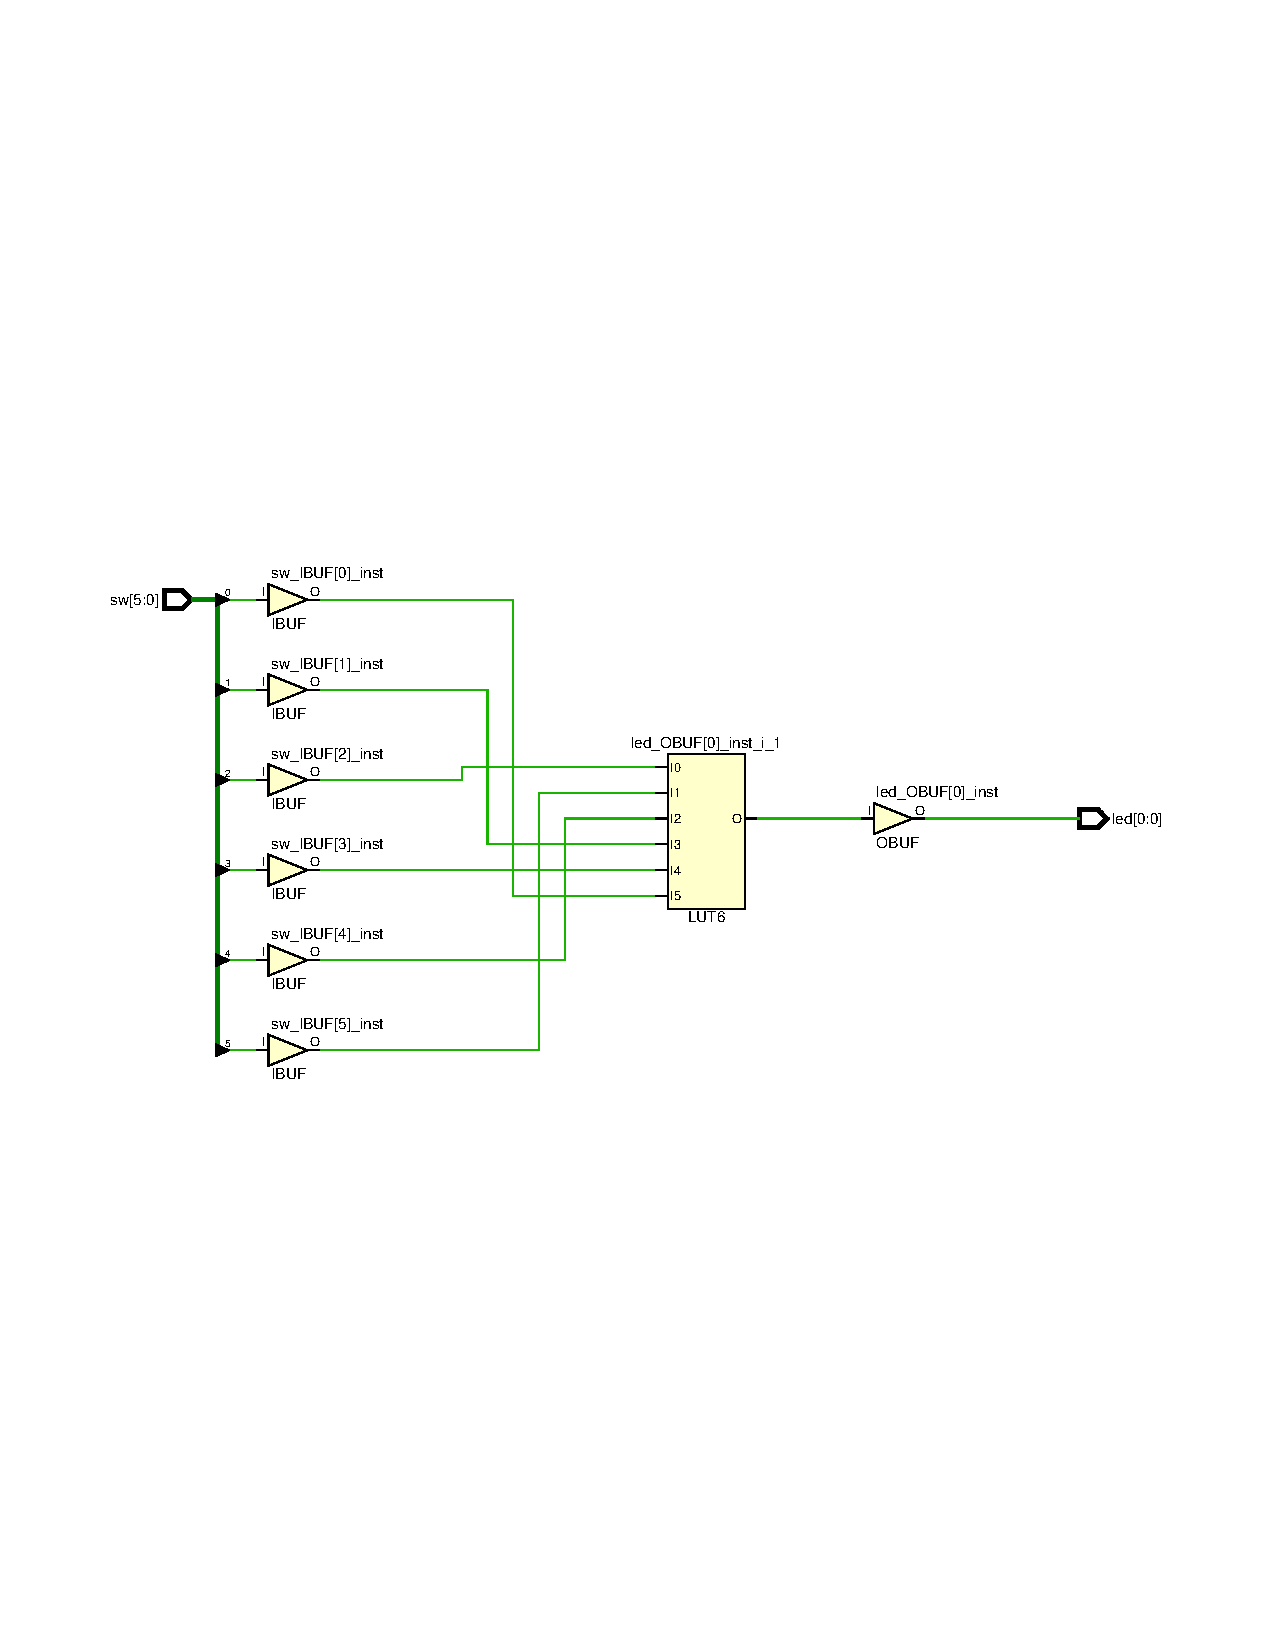
\includegraphics[width=\linewidth, trim=0mm 90mm 0mm 90mm]{./L1/E2/schematic.pdf}
	\caption{A schematic of the synthesized logic function.}
	\label{fig: schematic e_1_2_3}
\end{figure}

Just synthesizing the design leads to wrong mapped connections on the FPGA. Here, the buffers are not connected to any switches or the button. This can be easily fixed by adding a constraints file that matches the used board and renaming the ports accordingly.

\begin{figure}
	\centering
	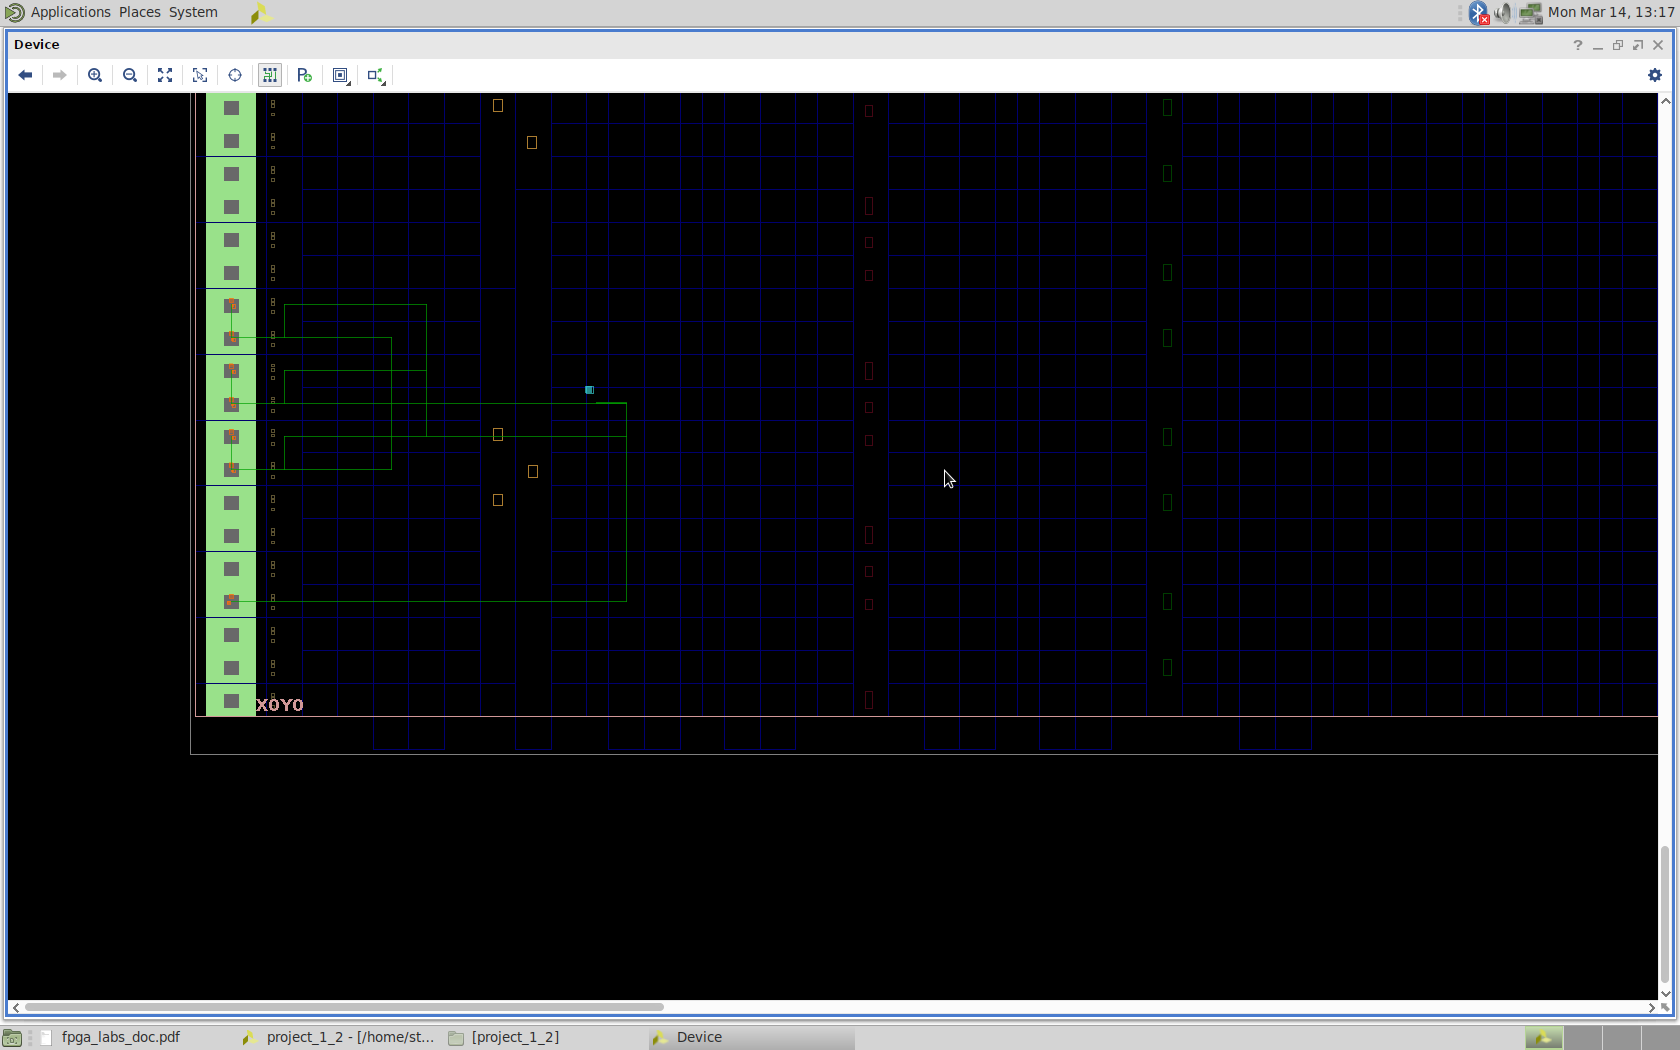
\includegraphics[width=.8\linewidth]{./L1/E2/step5}
	\caption{Placement design without constraints. The buffers are not connected to any ports and the connections are placed on arbitrary positions on the board.}
	\label{fig: placement without constraints e_1_2_4}
\end{figure}

\begin{figure}
	\centering
	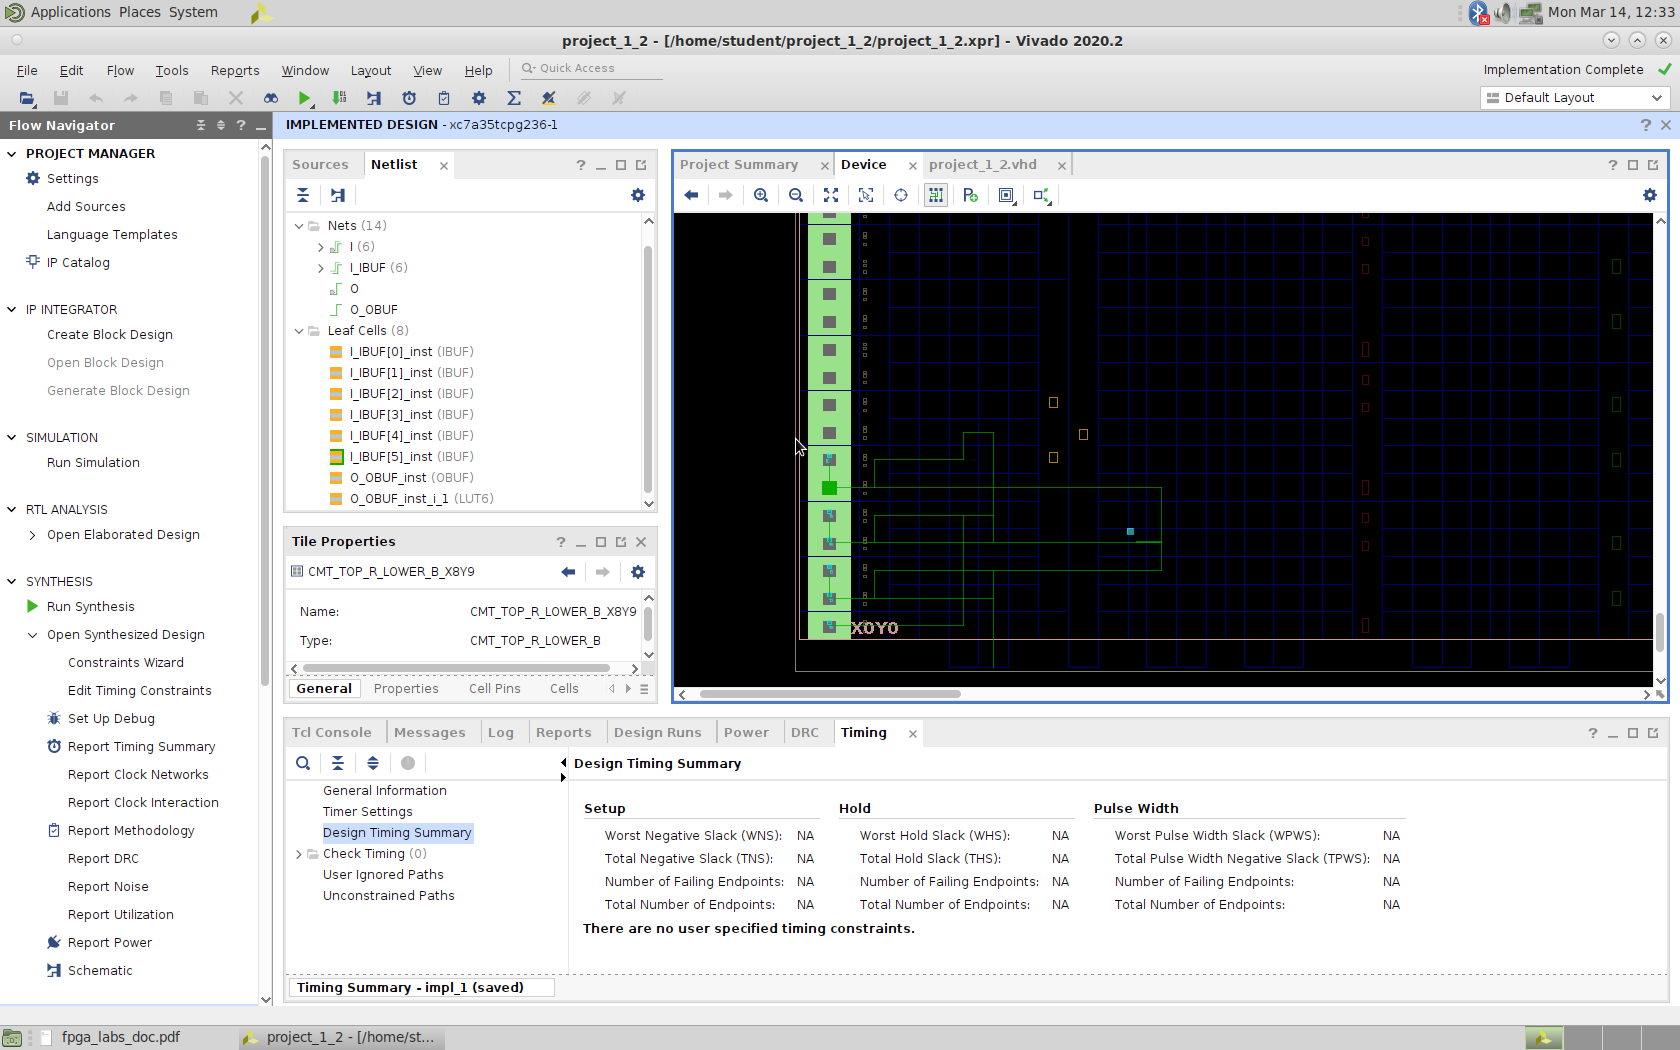
\includegraphics[width=.8\linewidth]{./L1/E2/with_constrains}
	\caption{Placement design with enabled constraints. Here the connections end on acutal ports.}
	\label{fig: placement with constraints e_1_2_5}
\end{figure}

\lstinputlisting[language=VHDL]{./L1/E3/src/Constraints_all.xdc}

\section{Parity Generator}

The third project of lab 1 is a parity generator that outputs a 1 if an odd number of switches is turned on or off and 0 for an even number. This was realized by concatenating the xor function.

\begin{figure}[h]
	\centering
	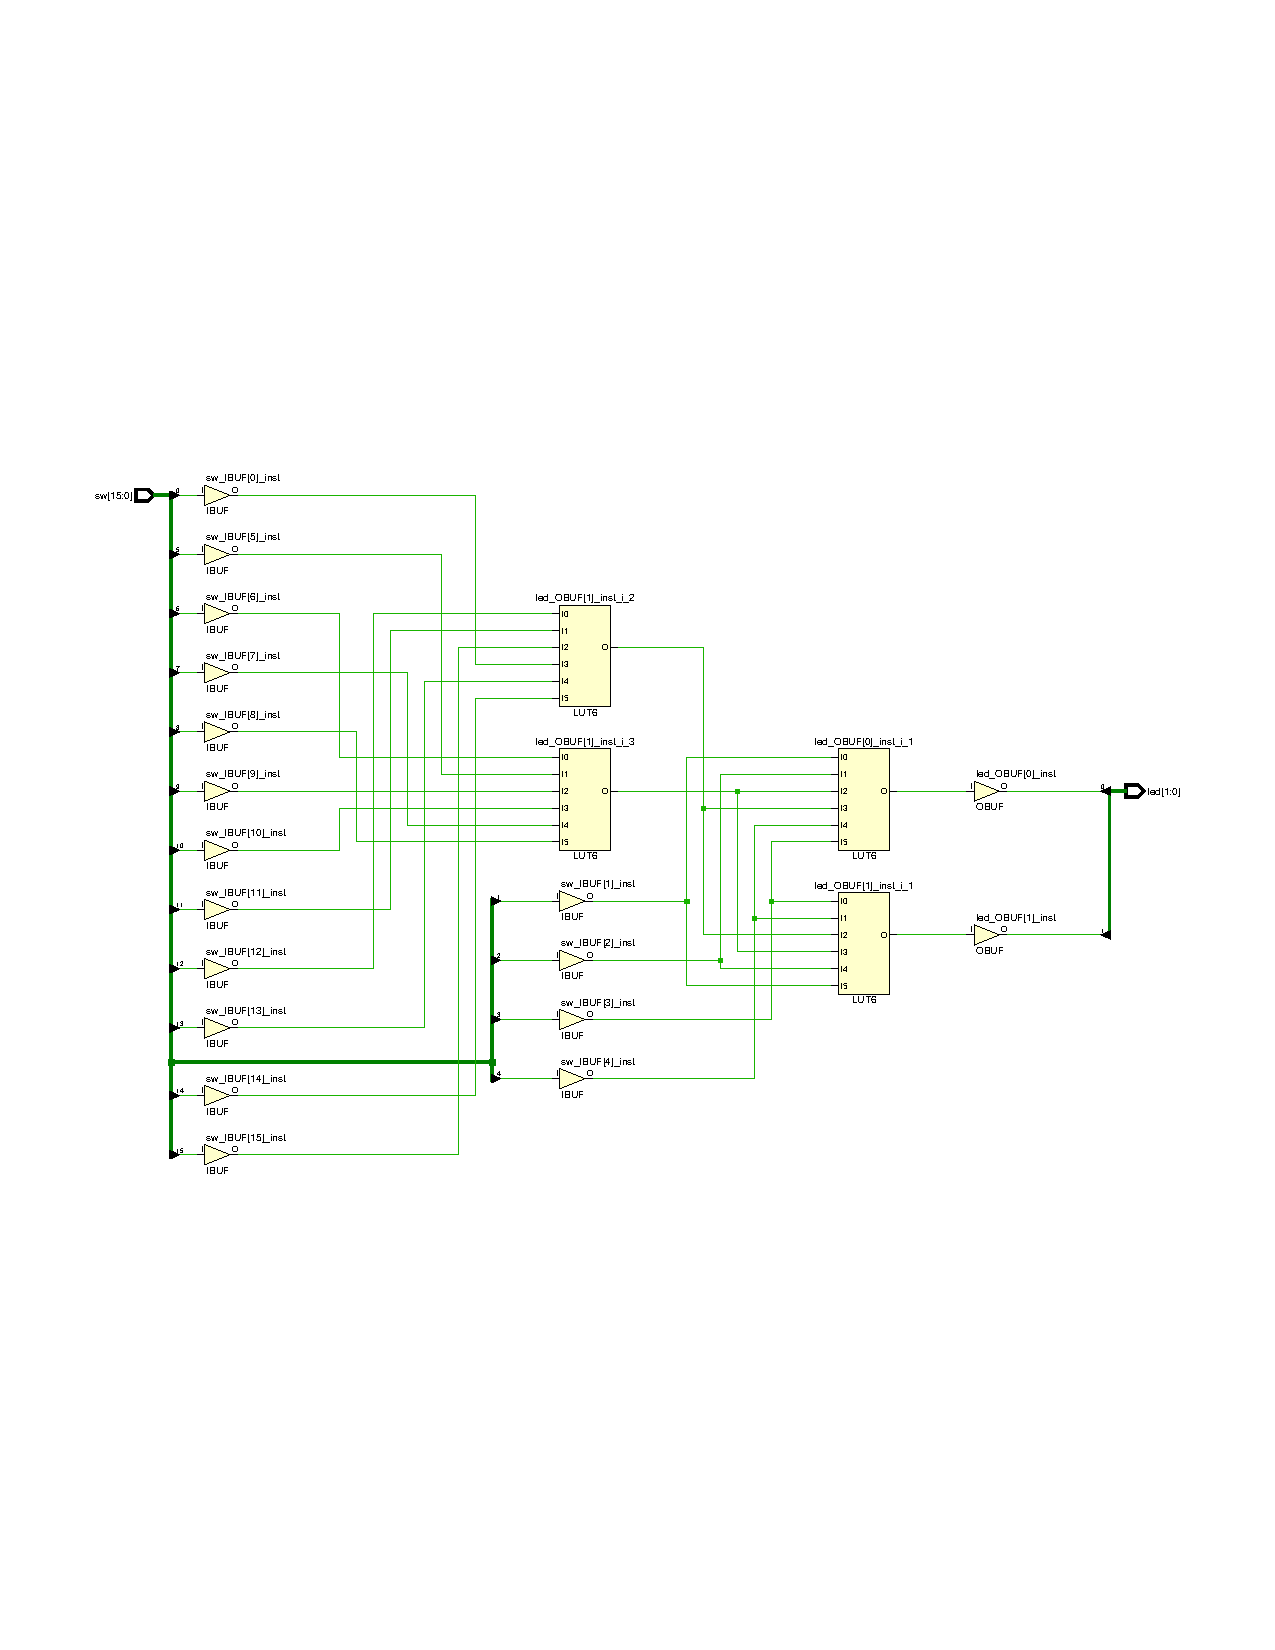
\includegraphics[width=\linewidth, trim=0mm 80mm 0mm 80mm]{./L1/E3/schematic.pdf}
	\caption{Schematic of the parity generator. This design uses four \glspl{lut}.}
	\label{fig: Parity Generator schematic}
\end{figure}

\lstinputlisting[language=VHDL]{./L1/E3/src/project_1_3.vhd}

\section{Full adder}

The full adder has three input switch and two output LEDs. Two of the three inputs are the bits that are added and the third one represents a carried bit from a previous addition. The two outputs represent one output bit and one bit that is to be carried on. 

\begin{figure}[h]
	\centering
	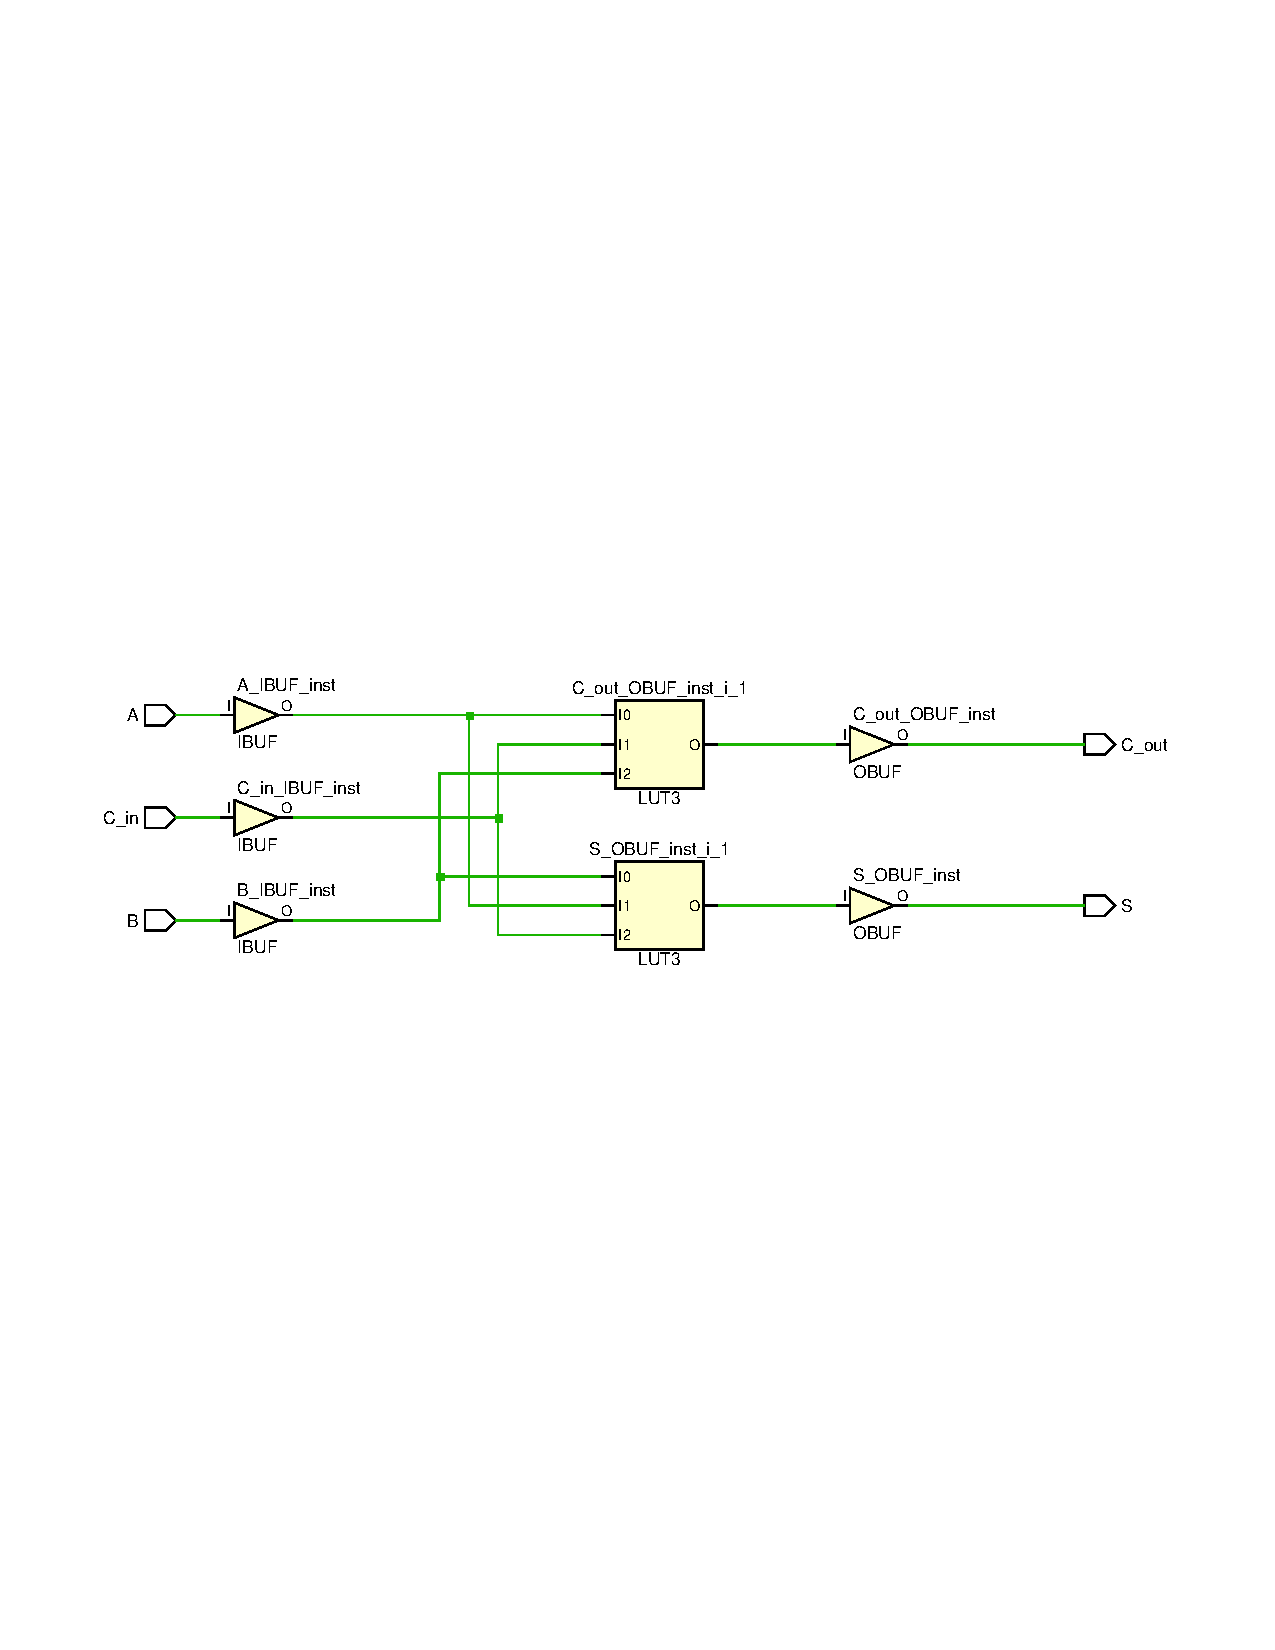
\includegraphics[width=\linewidth, trim=0mm 110mm 0mm 110mm]{./L1/E4/schematic.pdf}
	\caption{Schematic of the full adder. The synthesized design of the full adder uses two \glspl{lut} and buffers for every the in- and output. Both \glspl{lut} use just three of the six available inputs to add the three numbers and calculate the first bit of the result and the carried second bit, therefore two \glspl{lut} are needed to provide the two outputs.}
	\label{fig: Full Adder schematic}
\end{figure}

\lstinputlisting[language=VHDL]{./L1/E4/src/project_1_4.vhd}

\section{Ripple-carry adder}

The more advanced version of the previous adder is the ripple-carry adder. This is an adder composed of multiple full adders which enables the ripple-carry adder to add two 8-bit binary numbers.

\begin{figure}[h]
	\centering
	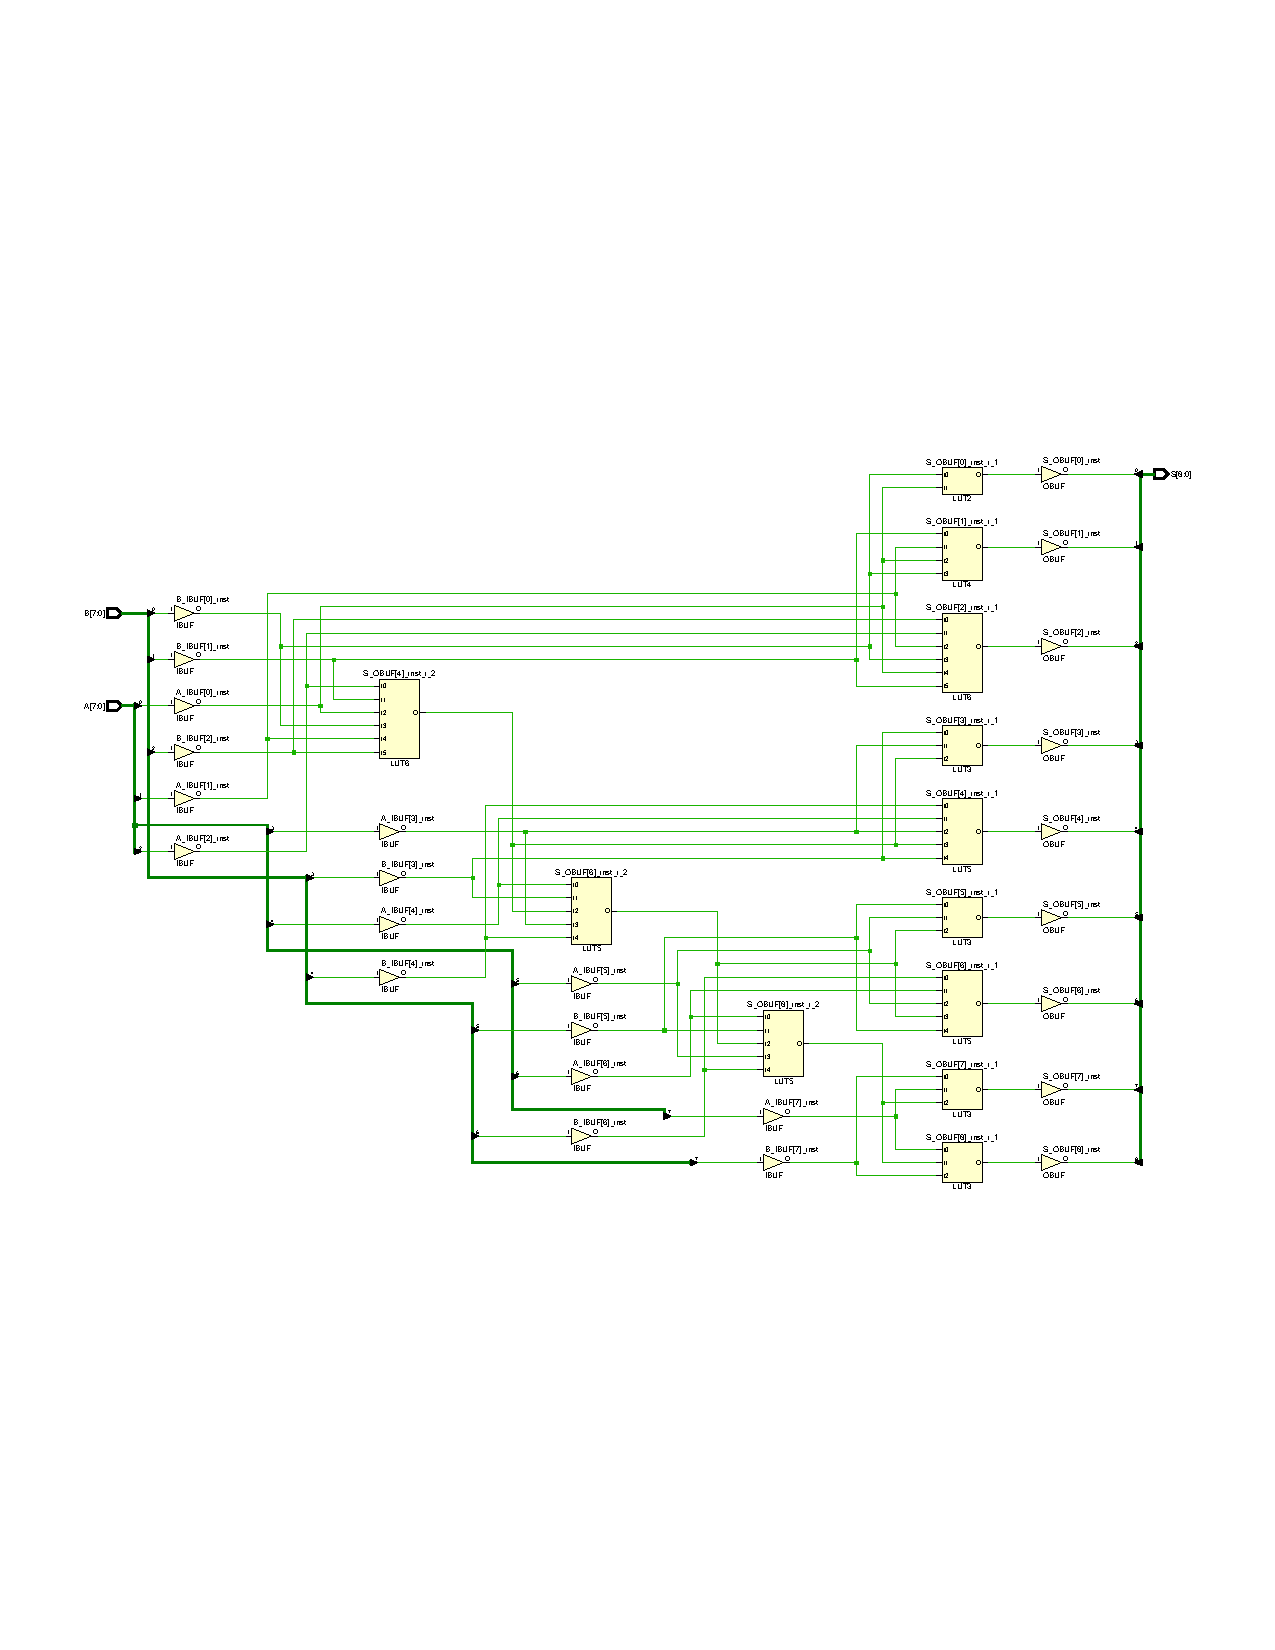
\includegraphics[width=\linewidth, trim=0mm 70mm 0mm 70mm]{./L1/E5/schematic.pdf}
	\caption{Schematic of the ripple-carry adder. This design again uses \glspl{lut} to realize the logic functions and buffers for the in- and outputs.}
	\label{fig: Ripple-carry adder schematic}
\end{figure}

\lstinputlisting[language=VHDL]{./L1/E5/src/project_1_5.vhd}

\lstinputlisting[language=VHDL]{./L1/E5/src/full_add.vhd}

\section{Inferring an adder from VHDL}

In this last project of this lab the ``ieee.numeric\_std.all'' library is used to code an adder. This is achieved with the ``unsigned'' data type. This data type can added with the ``+'' sign. The ``unsigned'' data type can be easily converted to a std\_logic\_vector and vice versa. 

\begin{figure}[h]
	\centering
	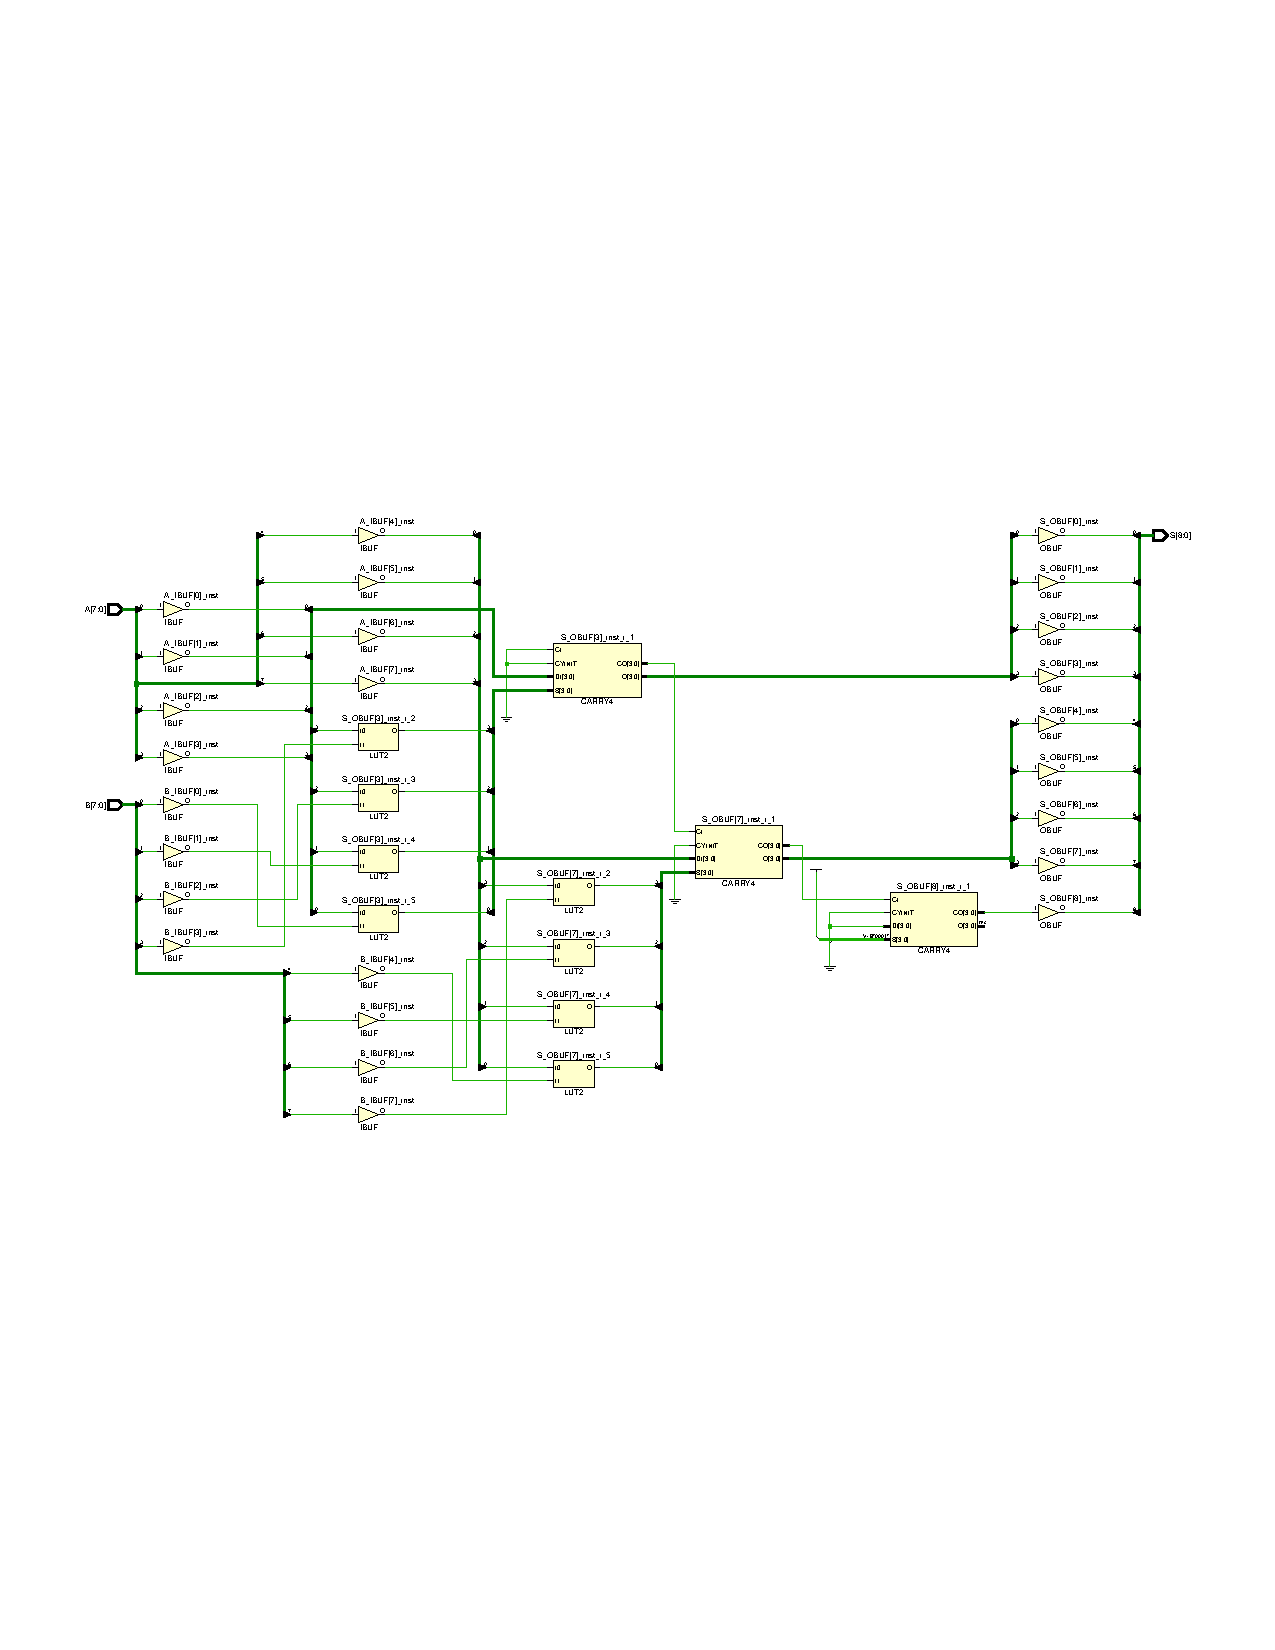
\includegraphics[width=\linewidth, trim=0mm 90mm 0mm 90mm]{./L1/E6/schematic.pdf}
	\caption{Schematic of the VHDL library adder. This design uses buffers as in- and outputs, \glspl{lut} and three carry logic blocks.}
	\label{fig: VHDL library adder}
\end{figure}

\lstinputlisting[language=VHDL]{./L1/E6/src/project_1_6.vhd}